
Fishing is central to the livelihood and food security of 200 million people, especially in developing countries, with one of five people depending on fish as the primary source of proteins (UN 2004). On the other hand, it is now widely recognized that fishing not only affects exploited species but the entire ecosystem in which they are embedded, highlighting the need for an ecosystem-based fisheries management (EBFM). By signing the Nagoya Strategic Plan of the Convention on Biological Diversity in October 2014, 50 nations and the European Union have committed to implement EBFM by 2020 (Aichi Biodiversity Target 6).However, the implementation of EBFM is still at its infancy worldwide. To be effective, EBFM not only requires a thorough understanding of the impact of fishing on ecosystem functioning and of the ecological processes involved, but also quantitative tools such as ecosystem models to provide useful information and predictions in support of management decision. Several marine ecosystem models have been implemented around the world (e.g., Ecopath with Ecosim, Atlantis, OSMOSE, etc.) and have the potential to be important tools for achieving EBFM goals as they incorporate species interactions and environmental forcing. Yet, the use of ecosystems models as decision making tools would only be possible if they are rigorously confronted to data by means of accurate and robust parameter estimation methods and algorithms (Bartell 2003). However, parameter estimation has been considered one of the two weakest points in ecological modeling as well as the ability of models to properly reflect the dynamic properties of the ecosystems (Jorgensen and Fath 2011).  

The Humboldt Current Ecosystem (HCE) is one of the four major Eastern Boundary Upwelling Systems of the Earth (with Canary, Benguela and California). It produces more fish per unit area than any other region in the world, and accounts for up to 10\% of the global fish catches (Chavez et al. 2008). The HCE has supported, on a long term basis, a fish production 20 times bigger than Canary or Benguela (Bakun and Broad 2003). The HCE extends from 4°S (northern Peru) to 40°S (central Chile), and its environmental variability is one of the highest in the world (Chavez et. al 2008), exhibiting a climatic and oceanographic variability at several scales (e.g. seasonal, interannual and decadal), the major source of interannual variability being the interruption of the upwelling seasonality by the El Nino Southern Oscillation ENSO (Alheit and Ñiquen 2004) which has direct effects on larval survival and fish recruitment success (Ñiquen and Bouchon 2004). Additionally, fishing activity can also be highly variable, depending on the variability in the abundance and accessibility of the main fishery resources like the Peruvian anchoveta (\emph{Engraulis ringens}). Thus, it is particularly crucial to better understand the impact of environmental variability and fishing on the most exploited small pelagic species, namely sardines and anchovies, because they are essential resources for the fishers and for the marine top predators of the HCE. The impacts of environmental variability may be propagated upwards through the food web by a progressive disruption in the phenological synchrony of species at adjacent trophic levels (Cury et al. 2008). In this context, understanding and quantifying the impacts of natural environmental variability on small pelagic fisheries and top predators requires integrated studies covering multiple trophic levels. 

In order to better understand the top-down effects of fishing and the bottom-up effects of natural climate variability and climate change on on the HCE, the objective of the thesis was to develop an integrated and multidisciplinary end-to-end (E2E) model of the HCE, including the explicit dynamics of the physical environment, the primary and secondary production, as well as the exploited fish communities. We conceived this E2E model so as to be possibly used in future as a tool for EBFM, adapted to the assessment and management of exploited fish populations, and allowing to better disentangle climate-driven from fishing impacts in the HCE. Therefore, we put emphasis in developing methods to rigorously confront the E2E model to observed data and increase its credibility.

The HCE E2E modeling first required to select and couple different component models together. To represent the High Trophic Level (HTL) community, we applied the spatially explicit individual-based model OSMOSE (Shin and Cury 2001, 2004) as the assumed opportunism in species interactions makes it relevant to use in a changing environment. Once the OSMOSE model properly structured and parameterized to the HCE , we coupled OSMOSE to an existing application of the ROMS-PISCES hydrodynamic and biogeochemical model (Aumont et al. 2003,Echevin et al. 2012) for representing explicitly the seasonal and interannual forcing from the Low Trophic Level (LTL) community and the physical environment. The resulting ROMS-PISCES-OSMOSE E2E model includes 13 species or functional groups: microphytoplankton, diatoms, microzooplankton, mesozooplankton, macrozooplankton, anchovy (\emph{Engraulis ringens}), sardine (\emph{Sardinops sagax}), jack mackerel (\emph{Trachurus murphyi}), horse mackerel (\emph{Scomber japonicus}), hake (\emph{Merluccius gayi}), munida (\emph{Pleurocondes monodon}), jumbo squid (\emph{Dosidicus gigas}) and mesopelagic fish. The difficulty of the thesis work was due to the combination of the strong technical issues related to the development of the E2E model, along with the conceptual representation of the entire HCE with inherent simplifications required on the selection and formulation of key processes. The former includes the necessity of using robust procedures for parameter estimation for a full calibration of the model, and the latter to find a good way to represent the interactions between the species and their environment. 

The OSMOSE model is a multispecies and Individual-based model (IBM) which focuses on fish species and HTL species in general, including invertebrate ones (Shin and Cury 2001, 2004). This model assumes size-based opportunistic predation that is conditioned by spatial co-occurrence and size adequacy between a predator and its prey. It represents fish individuals grouped in schools, which are characterized by their body size, weight, age, taxonomy and geographical location, and which undergo different processes over their life cycle (growth, explicit predation, natural and starvation mortalities, fishing mortality, reproduction and migration). In output, a variety of size-based and species-based ecological indicators can be simulated and confronted to in situ data (surveys and catch data) at different levels of aggregation. 

Physical processes in the HCE have been modeled with the ROMS (Regional Oceanic Modeling System, Shchepetkin and McWilliams 2003 and 2005 for more details), which simulated the climatological and interannual variation of temperature, salinity and currents off Peru (Penven et al. 2005, Colas et al. 2008). The outputs of ROMS have been used to force the PISCES (Pelagic Interaction Scheme for Carbon and Ecosystem Studies) biogeochemical model (Aumont et al. 2003). This model currently includes several components such as nutrients, phytoplankton, zooplankton and detritus (Aumont et al. 2003). The ROMS-PISCES model used as the LTL model in this thesis has been applied to the HCE with a spatial resolution of 1/6° and includes 2 size classes of phytoplankton, 2 size classes of zooplankton and 2 size classes of detritus, colimitations of phytoplankton growth by nitrate, phosphate, silicate and iron, and the oxygen cycle. The seasonal chlorophyll a variations in the HCE have been reproduced accurately using the ROMS-PISCES model (Echevin et al. 2008). 

The key coupling process used to link OSMOSE and ROMS-PISCES models is the predation process. The ROMS-PISCES model is used as a prey field for the OSMOSE model (concentration of nitrogen/carbon converted into wet biomass). Additionally, a significant contribution of the present thesis is to render explicit the link between fish habitats and the physical environment. Some of the outputs of the ROMS-PISCES model were used (e.g. plankton density, temperature, salinity, oxygen) to predict the spatial distribution of the species modelled in OSMOSE, by building climate niche models. The predictions of the statistical models were then incorporated into the OSMOSE model for each species.
A schematic representation of the coupling of OSMOSE and ROMS-PISCES is shown in Figure \ref{figure-E2E}.

\begin{figure}[t]
\centering 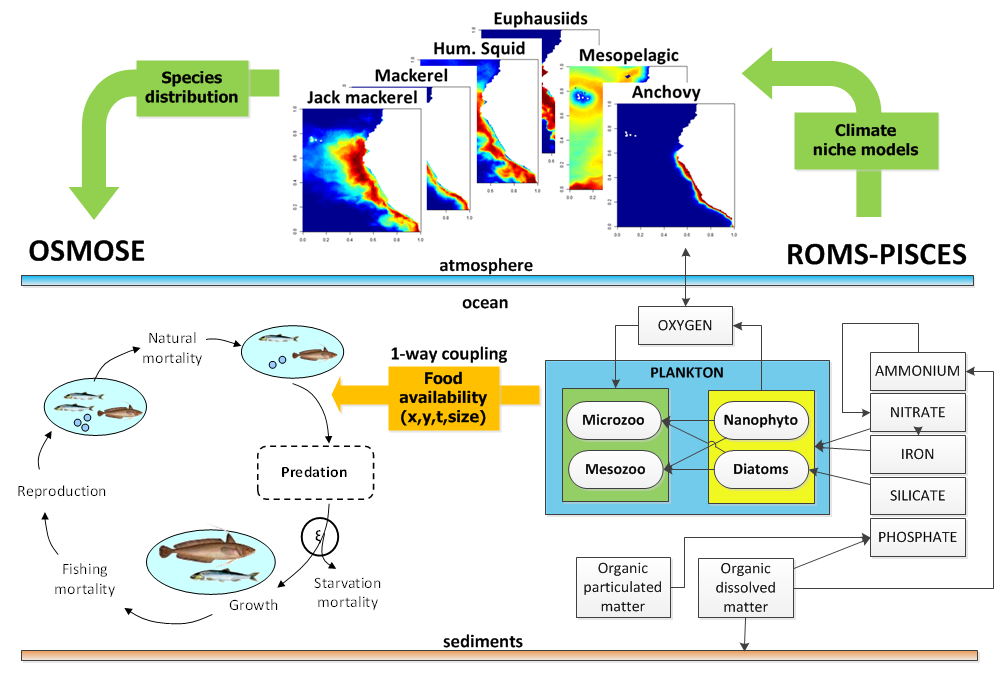
\includegraphics[width=0.9\textwidth]{figures/E2E_osmose}
\caption{Schematic representation of the key processes linking OSMOSE and ROMS-PISCES.}
\label{figure-E2E}
\end{figure}

Once the different pieces of the E2E model were assembled, an essential step consisted in calibrating the model using time series of data, and to do this rigorously, a specific algorithm had to be developed for the specific case of stochastic individual-based models (IBM). We significantly improved the convergence rate of a previous version of an evolutionary algorithm (Duboz et al. 2010) dedicated to OSMOSE calibration and we made the algorithm compatible with well-documented objective functions. In many respects, the calibration of ecosystem models such as OSMOSE is a complex task. In particular, the dynamics represented in ecosystem models allow species-specific parameters to have an impact on one another through ecological interactions, which results in highly correlated parameters, while additionally, critical information and observations on non-commercial species can be missing or poor. Furthermore, the high number of parameters and the long duration of the simulations can be an obstacle to calibrate a model. These diverse reasons hampered the development of flexible and generic enough calibration algorithms and methodologies for ecosystem models, and only sparse documentation has been produced on fitting complex models (Bolker et al. 2013). There are some dedicated tools for non-linear parameter estimation, AD Model Builder (ADMB, Fournier et al. 2012) being one of the most robust and fast (Bolker et al. 2013). Among other advantages, ADMB provides support for calibration in multiple phases (Nash and Walker-Smith 1987), which can be of great interest for the calibration of complex ecosystem models. It also provides support for constraining optimization, which can be helpful for regularizing hard optimization problems (Bolker et al. 2013). However, the model and the objective function itself need to be coded in C++ (using the ADMB scripting), which can be an obstacle for calibrating complex models already implemented in other languages (e.g. Java, Fortran). In addition, as ADMB is based on automatic differentiation, which allows to provide accurate estimates of derivatives (Griewank and Corliss 1992), the tool is not suited for stochastic models for which derivatives cannot be computed, like Individual Based Models (IBM). Parameter estimation methods have been developed for stochastic non-linear models for which the probability of state transitions or the master equation can be written (Ionides et al. 2006, Newman et al. 2009, Ross et al. 2009, Walker et al. 2006). However, many IBMs can only be simulated numerically and are too complex for mathematical analysis and explicit parameter estimation (Black and McKane 2012), resulting in more attention being given to the exploration of model behavior than to a rigorous confrontation with data. As alternative methods, meta-heuristic algorithms have been developed (Cropper and Anderson 2004, Poovathingal and Gunawan 2010, Duboz et at. 2010, Tashkova et al. 2012, Travers-Trolet et al. 2013), and have in some cases shown better performance than derivative-based optimization methods (Tashkova et al. 2012). However, the scientific community lacks generic and flexible enough tools for the calibration of different types of ecological models with different degrees of complexity. In this respect, a major part of this thesis has been dedicated to the conceptual and technical development of calibrar, an R package (R Development Core Team 2014) for the calibration of complex models, in particular stochastic ones. The main features of this software are shown in Figure 2.


\begin{figure}[t]
\centering 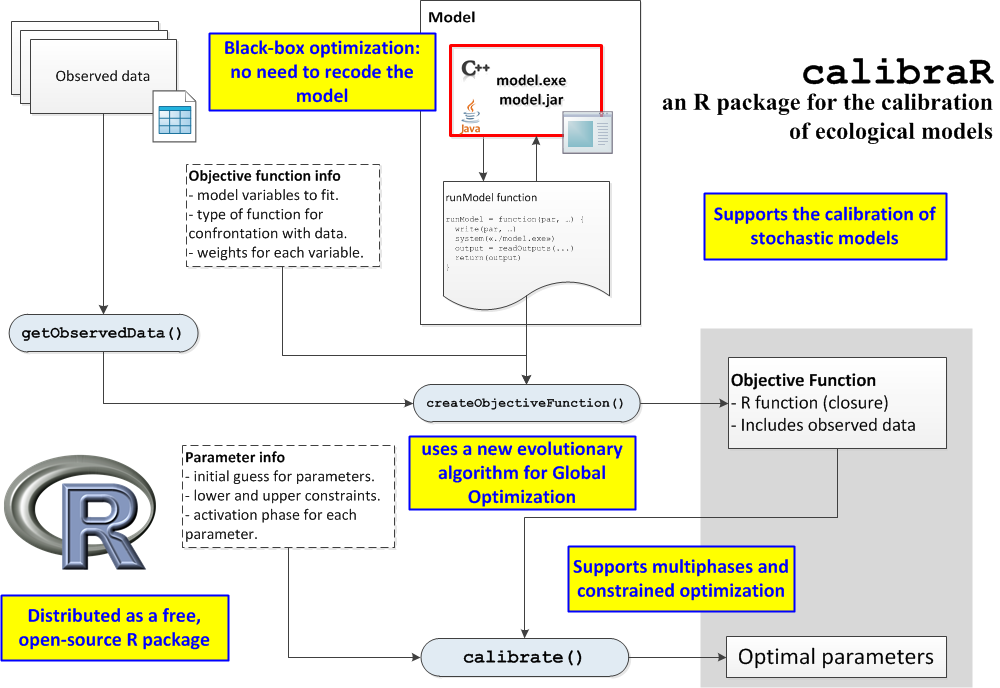
\includegraphics[width=0.9\textwidth]{figures/calibraR}
\caption{Diagram representing the functioning of the calibrar package. The grey area groups the outputs produced for the package (the objective function and the optimal parameters of the model). Rectangles with broken border lines show user inputs which are needed to configure the calibration. Rounded rectangles show main package functions.}
\label{figure-calibrar}
\end{figure}

Given that the calibration of complex ecosystem models requires a lot of data and potentially involves a high number of parameters to estimate, common practice in the field has been to i) reduce the number of parameters to estimate by using estimates provided by other models (Marzloff et al. 2009, Lehuta et al. 2010) or available for similar species or ecosystems (Bundy 2005, Ruiz and Wolff 2011), ii) use other models outputs as data to calibrate the model (Mackinson and Daskalov 2007), or both (Shannon et al. 2003, Guénette et al. 2008, Friska et al. 2011, Travers-Trolet et al. 2013). These different strategies allow to calibrate complex models while attempting to synthesize the maximum of available information. However, as the parameters or outputs used rely on different model assumptions, they may lead to the fitting of artificial parameter values or to inconsistent behavior of the model by trying to reproduce other models' dynamics. Additionally, ecosystem models can require more information to be built, information which may not normally be available (e.g distribution maps for all species). This lack of information is particularly true for non-commercial species or when information required is outside the Economic Exclusive Zone of the countries involved. This situation can limit the development of ecosystem models to areas rich in data. Additional issues can however be raised even in data-rich situations, since the reconstruction of valid spatial information to drive the models is not straightforward.

All these challenges were addressed in this thesis, with the objective to build an end-to-end (E2E) model of the HCE in order to investigate the impacts of environmental variability and fishing scenarios on the management of fishery resources. In the process, the HCE proved to be an ideal model case study to address these issues, as it is a well-studied ecosystem with long time-series of data for species at multiple trophic levels. The main outcomes of this thesis are presented in three chapters and some general conclusions and perspectives are finally drawn to pave the way for future work.

In Chapter 1, we describe the development of an end-to-end model of the Northern Humboldt Current Ecosystem, by coupling ROMS-PISCES and OSMOSE models. We particularly deal with the incorporation of the impact of the interannual variability of the environment and fishing as part of the process of constructing our E2E model. One of the main interannual forcing in OSMOSE is the spatial distribution of fish and other modelled species that we incorporated by building ecological niche models. These models were used to produce monthly maps of spatial distribution for all the species included in our model. For the validation of these niche models, typically based on the classification or regression of binary presence/absence data against several environmental or geographical variables, the confusion matrix and the statistical metrics associated to it are normally used. However, when considering the prediction of the habitat against time, the variability in the spatial distribution of the habitat can be summarized and validated using the emerging patterns from the shape of this distribution. To illustrate this approach, we used jack mackerel (\emph{Trachurus murphyi}) spatial distribution results. The potential habitat was predicted over the study period with monthly resolution, and the model was validated using quantitative and qualitative information of the system compared with i) one dimensional profiles inside the scientific survey area (latitudinal and off-shore distributions) and, ii) time series of the center of gravity of the spatial distribution, modes, quantiles and extremes of the profiles (Manuscript 1: Oliveros et al. in prep). 

In Chapter 2 we present an optimization method that we developed for the calibration of stochastic models, OSMOSE in particular (Manuscript 2: Oliveros and Shin, in review). The calibration algorithm is an Evolutionary Strategy (Beyer and Schwefel 2002) and its implementation as well the tools related to the calibration have been implemented in a package, \texttt{calibrar}, written in R (R Development Core Team 2014). The \texttt{calibrar} package is designed for the optimization of “black-box” functions (Jones et al. 1998), where analytical information about the function to be optimized and the model source code are assumed to be unavailable or impractical to modify (Rios and Sahinidis 2013). Our approach is hence “non-intrusive”, making the model interact with the optimizer, i.e. the \texttt{calibrar} package, in two ways: i) receiving a set of parameters to run, and ii) providing the model outputs to be confronted with the observed data. \texttt{calibrar}also helps in the construction of the objective function to be optimized in order to estimate model parameters (Figure \ref{figure-calibrar}).

In Chapter 3 we propose an approach to deal with the calibration of ecosystem models, and we illustrate it with the end-to-end (E2E) ecosystem model ROMS-PISCES-OSMOSE of the Northern Humboldt Current Ecosystem. Here, we highlight some issues related to the confrontation of complex ecosystem models to data and propose a methodology for a sequential multi-phases calibration of ecosystem models (Manuscript 3: Oliveros et al. in review). We first discuss two criteria to classify the parameters of a model: the model dependency and the time variability of the parameters. Then, these criteria and the availability of approximate initial estimates are used as decision rules to determine which parameters need to be estimated, and their precedence order in the sequential calibration process. The \texttt{calibrar}R package and a likelihood approach are used to fit  monthly time series data of landings, abundance indices and catch at length distributions from 1992 to 2008. 

Finally, we conclude with some perspectives brought out by our work, and particularly on how ecosystem models can be used in the context of the Ecosystem Approach to Fisheries to complement the assessment and recommendations based on single-species models for fishery management.

\section*{References}

Alheit J., Ñiquen M., 2004. Regime shifts in the Humboldt Current ecosystem. Progress in Oceanography 60:201–222.

Aumont, O. E. Maier-Reimer, S. Blain and P. Monfray. 2003. An ecosystem model of the global ocean including Fe, Si, P colimitations. Global Biogeochemical Cycles, (17) 1060.

Bakun, A. and K. Broad., 2003. Environmental loopholes and fish population dynamics: comparative pattern recognition with focus on El Niño effects in the Pacific. Fisheries Oceanography. 12(4/5):458-473.

Beyer, H.-G. and Schwefel, H.-P., 2002. Evolution strategies: a comprehensive introduction, Natural Computing 1:3-52.

Black, A.J. andMcKane, A.J., 2012. Stochastic formulation of ecological models and their applications. Trend in Ecology and Evolution 27(6):337-345. DOI: http://dx.doi.org/10.1016/j.tree.2012.01.014

Bartell S.M., 2003. Effective use of ecological modeling in management: The toolkit concept. In Dale V (editor).Ecological modeling for resource management, Springer Verlag.

Bolker B.M., Gardner B., Maunder M., Berg C.W. , Brooks M., Comita L., Crone E., Cubaynes S., Davies T., de Valpine P., Ford J., Gimenez O., Kéry M., Kim E.J., Lennert-Cody C., Magnusson A., Martell S., Nash J., Nielsen A., Regetz J., Skaug H., Zipkin E., 2013. Strategies for fitting nonlinear ecological models in R, AD Model Builder, and BUGS. Methods in Ecology and Evolution 4: 501–512.

Bundy A., 2005.  Structure and functioning of the eastern Scotian Shelf ecosystem before and after the collapse of ground fish stocks in the early 1990s. Canadian Journal of Fisheries And Aquatic Sciences 62:1453-1473.

Chavez F. P., A. Bertrand, R. Guevara-Carrasco, P. Soler and J. Csirke. 2008. The northern Humboldt Current System: Brief history, present status and a view towards the future. Progress in Oceanography 79:95-105.

Colas F., X. Capet, J.C. McWilliams and A. Shchepetkin. 2008. 1997-1998 El Niño off Peru: A numerical study. Progress in Oceanography 79:138-155. 

Cropper, W.P. Jr. and Anderson, P.J., 2004. Population dynamics of a tropical palm: use of a genetic algorithm for inverse parameter estimation. Ecological Modelling 177: 119–127.

Cury PM, Shin Y-J, Planque B, Durant JM, Fromentin J-M, Kramer-Schadt S, Stenseth NC, Travers M and Grimm V (2008) Ecosystem oceanography for global change in fisheries. Trends in Ecology and Evolution 23:338-346

Duboz, R., Versmisse, D., Travers, M., Ramat, E. and Shin, Y.-J., 2010. Application of an evolutionary algorithm to the inverse parameter estimation of an individual-based model. Ecological Modelling 221(5):840-849.

Echevin V., O. Aumont, J. Ledesma, G. Flores. 2008. The seasonal cycle of surface chlorophyll in the Peruvian upwelling system: A modelling study. Progress in Oceanography 79:167-176.

Echevin V., Goubanova K., Dewitte B., Belmadani A., 2012. Sensitivity of the Humboldt Current system to global warming: a downscaling experiment of the IPSL-CM4 model, Climate Dynamics. doi:10.1007/s00382-011-1085-2.

Fournier D.A., Skaug H.J., Ancheta J., Ianelli J., Magnusson A., Maunder M.N., Nielsen A., Sibert J., 2012. AD Model Builder: using automatic differentiation for statistical inference of highly parameterized complex nonlinear models. Optimization Methods and Software, 27:2, 233-249, DOI: 10.1080/10556788.2011.597854.

Friska M.G., Miller T.J., Latour R.J., Martell S.J.D., 2011. Assessing biomass gains from marsh restoration in Delaware Bay using Ecopath with Ecosim. Ecological Modelling 222:190–200.

Garcia, S.M.; Zerbi, A.; Aliaume, C.; Do Chi, T.; Lasserre, G. 2003. The ecosystem approach to fisheries. Issues, terminology, principles, institutional foundations, implementation and outlook. FAO Fisheries Technical Paper. No. 443. Rome, FAO. 71 p.

Griewank, A. and Corliss, G.F., 1992. Automatic Differentiation of Algorithms: Theory, Implementation, and Application. SIAM, Philadelphia, PA, USA.

Guénette S., Christensen V., Pauly D., 2008. Trophic modelling of the Peruvian upwelling ecosystem: Towards reconciliation of multiple datasets. Progress in Oceanography 79: 326–335.

Ionides, E. L., Breto, C. and King, A.A., 2006. Inference for nonlinear dynamical systems. PNAS 103(49): 18438–18443.

Jones, G. (1998) Genetic and evolutionary algorithms. In Encyclopedia of Computational Chemistry (Schleyer, P .v.R. et al., eds), pp. 1127–1136, John Wiley \& Sons.

Jorgensen S.E. and FathB.D., 2011. Fundamentals of Ecological Modelling: Applications in Environmental Management and Research. Fourth Edition. Elsevier. 350pp.

Lehuta S., Petitgas P., Mahévas S., Huret M., Vermard Y., Uriarte A.,  Record N.R.,  2013. Selection  and  validation  of  a  complex  fishery  model  using  an  uncertainty hierarchy. Fisheries  Research  143:57–  66.

Mackinson S., and Daskalov G., 2007. An ecosystem model of the North Sea for use in research supporting the ecosystem approach to fisheries management: description and parameterisation [online]. (CEFAS, Lowestoft.) Available from www.cefas.co.uk/publications/techrep/tech142.pdf. 

Marzloff M., Shin Y.-J., Tam J., Travers M., Bertrand A., 2009. Trophic structure of the Peruvian marine ecosystem in 2000–2006: Insights on the effects of management scenarios for the hake fishery using the IBM trophic model Osmose. Journal of Marine Systems 75: 290-304.

Nash J.C. and Walker-Smith M., 1987. Nonlinear Parameter Estimation: an Integrated System in BASIC. Marcel Dekker, New York. 493pp.

Newman, K.B., Fernández, C., Thomas, L. and Buckland, S.T., 2009. Monte Carlo Inference for State–Space Models of Wild Animal Populations. Biometrics 65, 572–583.

Ñiquen M., Bouchon M., Ulloa D., Medina A., 2013. Analysis of the Jack mackerel Trachurus murphyi fishery in Peru. Rev. Peru. Biol. 20(1):097-106. 

Penven, P., V. Echevin, J. Pasapera, F. Colas, J. Tam. 2005. Average circulation, seasonal cycle, and mesoscale dynamics of the Peru Current System: A modeling approach. J. Geophys. Res., Vol. 110, No. C10, C1002110.1029/2005JC002945.

Poovathingal, S.K andGunawan, R., 2010. Global parameter estimation methods for stochastic biochemical systems, BMC Bioinformatics 11:414. 

R Core Team (2014) R: A language and environment for statistical computing. R Foundation for Statistical Computing, Vienna, Austria. URL http://www.R-project.org/.

Rios, L.M. \& Sahinidis, N.V. (2013) Derivative-free optimization: a review of algorithms and comparison of software implementations. Journal of Global Optimization 56:1247–1293.

Ross, J.V., Pagendam, D.E. andPollet P.K., 2009. On parameter estimation in population models II: Multi-dimensional processes and transient dynamics. Theoretical Population Biology 75: 123132.

Ruiz D.J, Wolff M., 2011. The Bolivar Channel Ecosystem of the Galapagos Marine Reserve: Energy flow structure and role of keystone groups. Journal of Sea Research 66 123–134.

Shannon L.J., Moloney C.L., Jarre A., Field J.G., 2003. Trophic flows in the southern Benguela during the 1980s and 1990s. Journal of Marine Systems 39:83 – 116.

Shchepetkin, A. F., and J. C. McWilliams, 2003. A method for computing horizontal pressure-gradient force in an ocean model with a nonaligned vertical coordinate, J. Geophys. Res.,108 (C3), 3090, doi:10.1029/2001JC001047.

Shchepetkin, A. F., and J. C. McWilliams, 2005. The regional oceanic modeling system (ROMS): A split-explicit, free-surface, topography-following-coordinate oceanic model, Ocean Modell., 9 , 347–404.

Shin Y.-J., P. Cury. 2001. Exploring fish community dynamics through size-dependent trophic interactions using a spatialized individual-based model. Aquatic Living Resources, 14(2): 65-80.

Shin Y.-J., P. Cury, 2004. Using an individual-based model of fish assemblages to study the response of size spectra to changes in fishing. Canadian Journal of Fisheries and Aquatic Sciences, 61: 414-431.

Tashkova, K., Silc, J., Atanasova, N. andDzeroski, S., 2012. Parameter estimation in a nonlinear dynamic model of an aquatic ecosystem with meta-heuristic optimization. Ecological Modelling 226: 36– 61.

Travers-Trolet, M., Shin, Y.-J. and Field, J.G., 2013. An end-to-end coupled model ROMS-N2P2Z2D2-OSMOSE of the southern Benguelafoodweb: parameterisation, calibration and pattern-oriented validation, African Journal of Marine Science, 36:1, 11-29,  DOI:10.2989/1814232X.2014.883326

United Nations. 2004. Overfishing: a threat to marine biodiversity. “Ten Stories the World Should Know More About.” http://www.un.org/events/tenstories/

Walker, D.M., Pérez-Barbería, F.J. and Marion, G., 2006. Stochastic modelling of ecological processes using hybrid Gibbs samplers. Ecological Modelling 198:40-52.



